\documentclass{article}
\usepackage[utf8]{inputenc}
\usepackage{geometry}
\usepackage{graphicx}
\geometry{hmargin=2.5cm,vmargin=1.5cm}

\title{Challenge - Prévision}
\author{Stephani Ujka}
\date{Le 1$^{er}$ avril 2021}

\begin{document}

\maketitle

\paragraph{Nous voulons prédire le nombre de vélos passant entre 00h01 et 9h00 le vendredi 2 avril 2021 à Albert 1er, à Montpellier. Nous avons utilisé une méthode couramment utilisée pour la prédiction des séries temporelles : SARIMA. Mais avant, nous devons nettoyer les données pour  les exploiter.}

\section{Notre base de données}

Nous avons supprimé des colonnes vides, d'autres inutiles, renommé des colonnes de manière plus 'lisible', reformaté les dates. Nous avons mis en index la date et l'heure.\\

En raison de la crise de la covid en 2020, entre confinements et couvre-feux, la situation en France n'était pas très stable. Nous avons décidé de ne prendre que les données à partir du 17 janvier 2021, date de la dernière décision politique mise en application : le couvre-feux de 18h00 à 6h00.\\
Nous avons également filtré ce dernier jeu de données en ne prenant que la plage horaire 00h01-9h01 (rajout d'une minute pour gagner une donnée, car il n'en reste déjà plus beaucoup).\\
Enfin, nous avons traité les données manquantes suivant le jour de la semaine. Du lundi au vendredi, nous avons pris la médiane des données en semaine. Le samedi et le dimanche, nous avons utilisé la moyenne des données en week-end.
\begin{figure}[h]
    \centering
    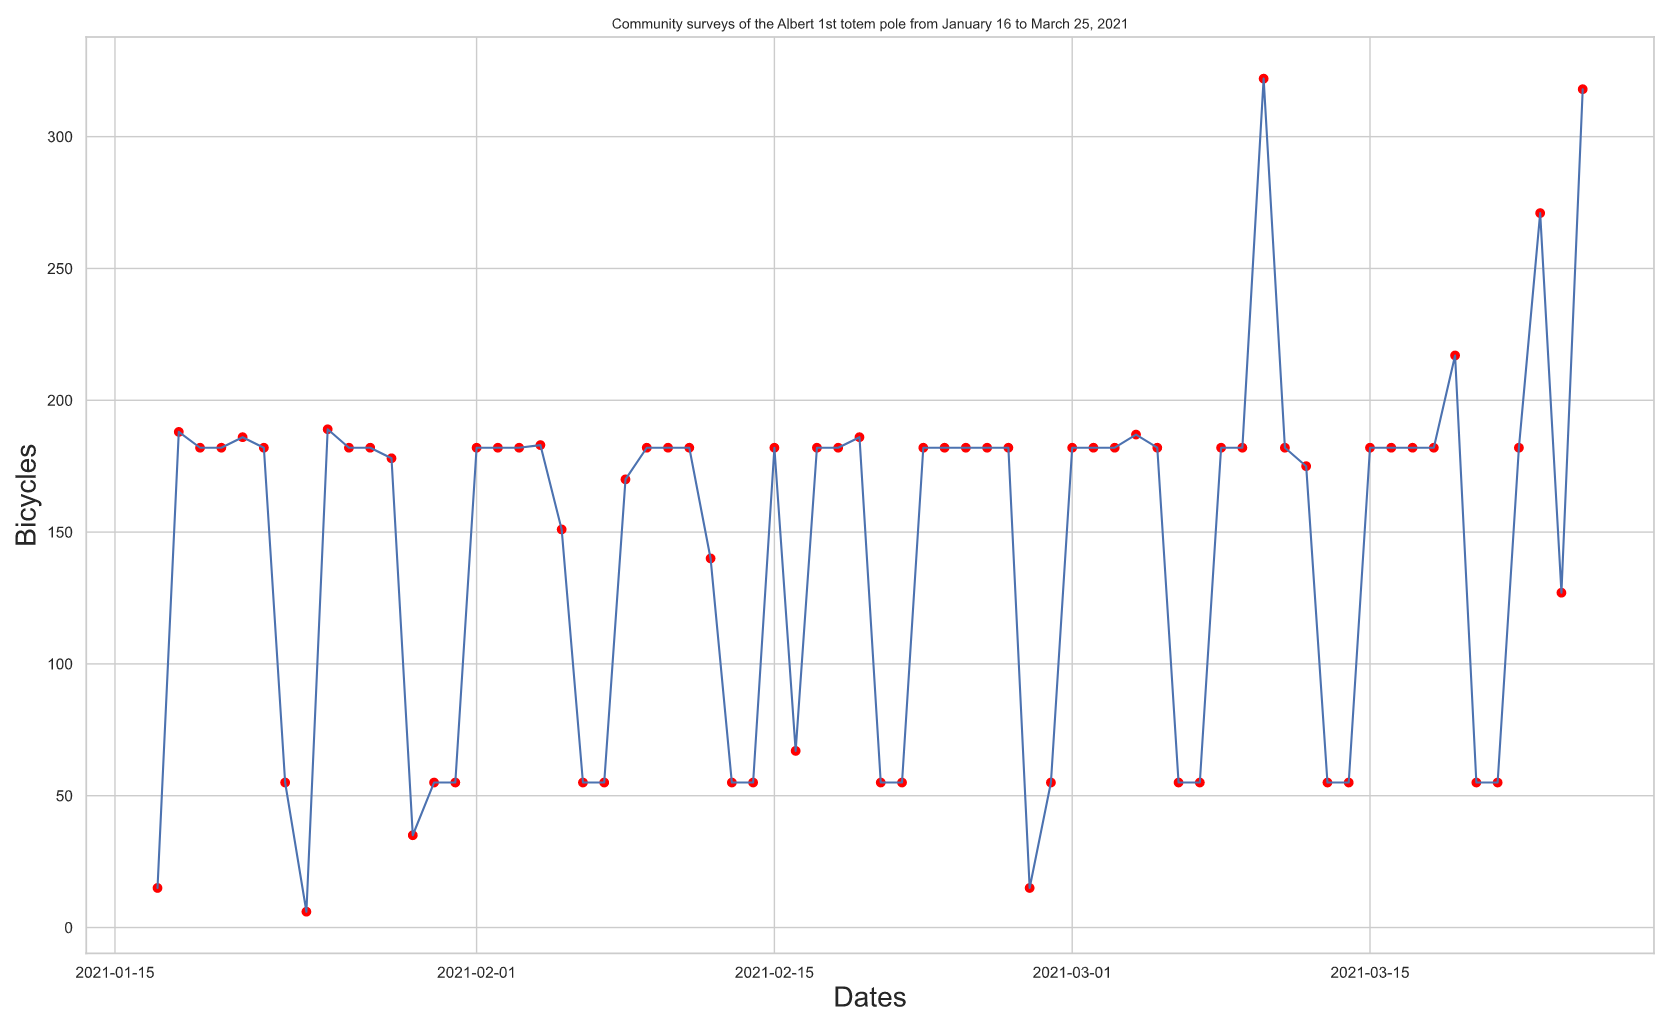
\includegraphics[scale=0.5]{data1.png}
\end{figure}
\newpage
\section{Méthode SARIMA}

\subsection{Optimalité du modèle}

\begin{figure}[h]
    \centering
    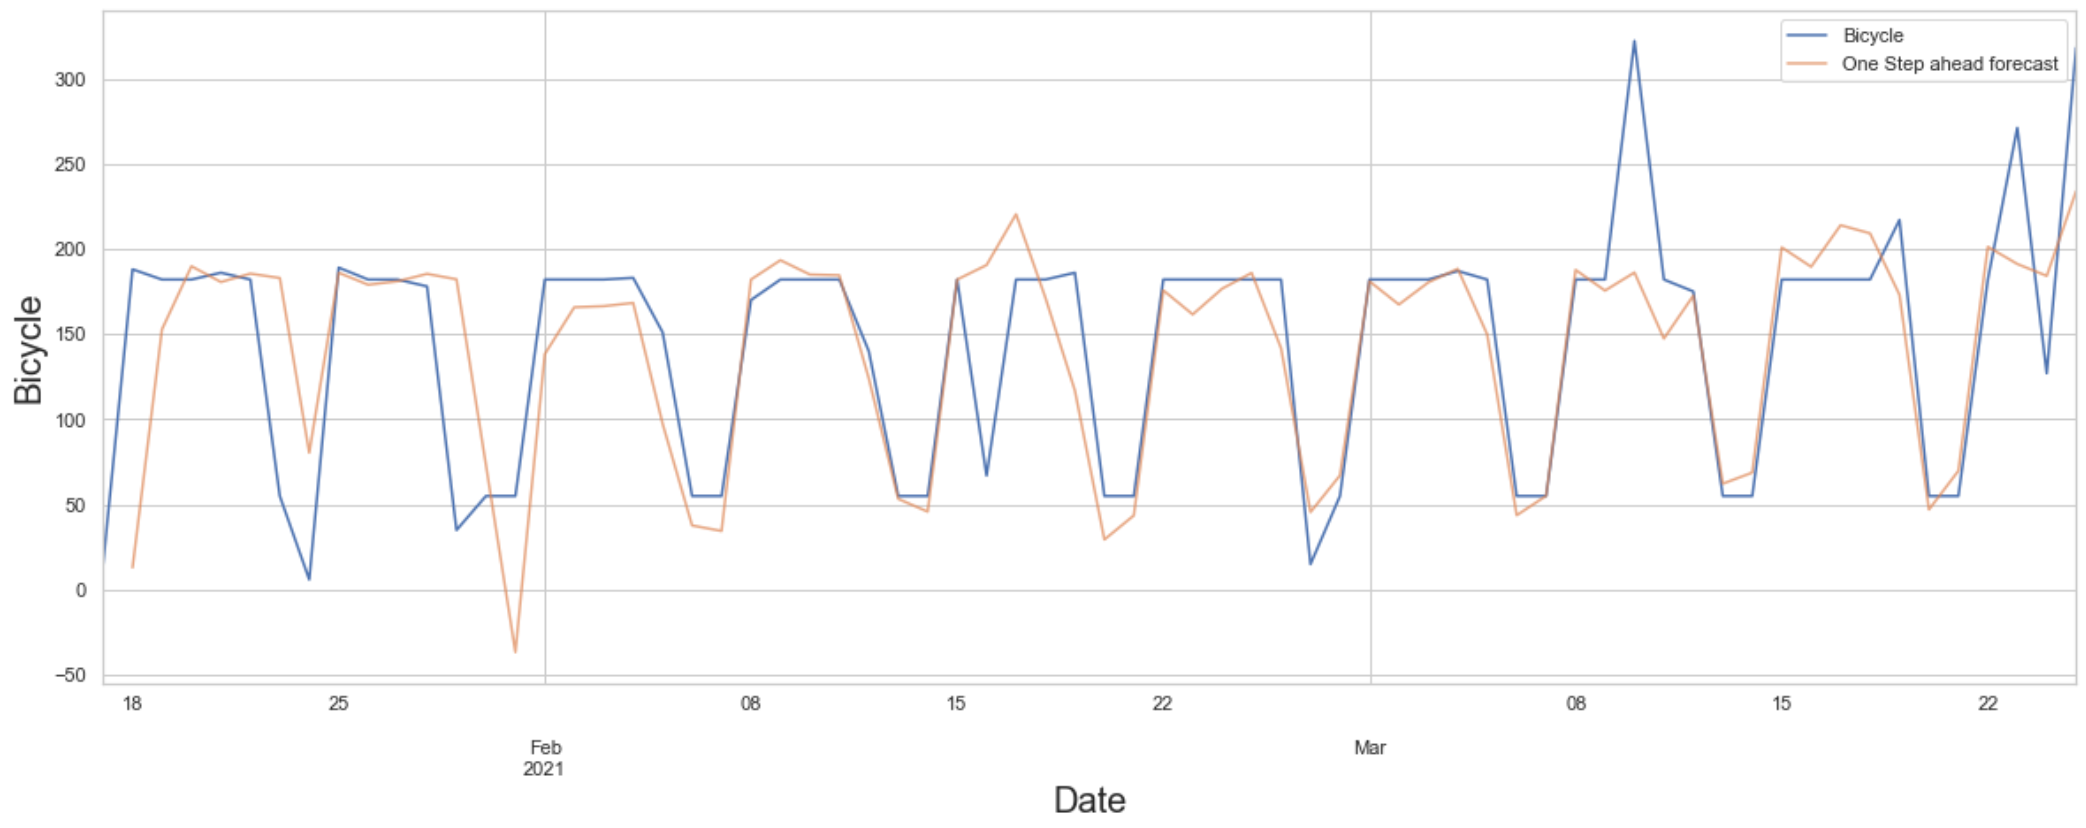
\includegraphics[scale=0.4]{data2.png}
\end{figure}

\subsection{Prévision sur 25 jours}

\begin{figure}[h]
    \centering
    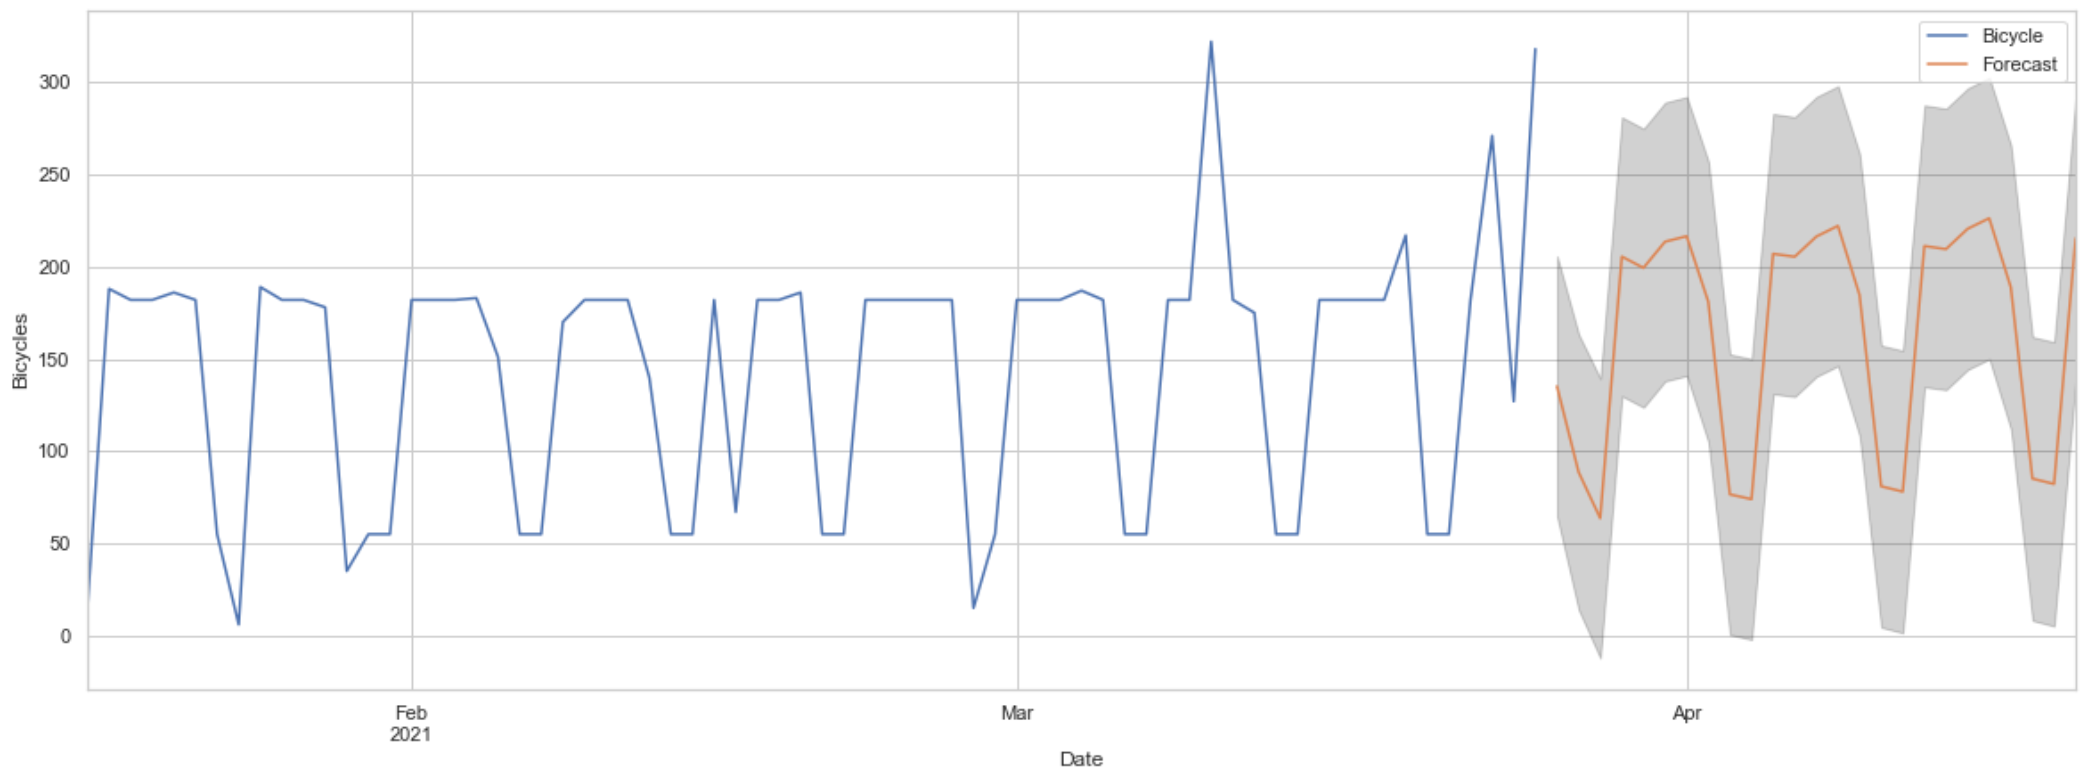
\includegraphics[scale=0.4]{data3.png}
\end{figure}

\begin{figure}[h]
    \centering
    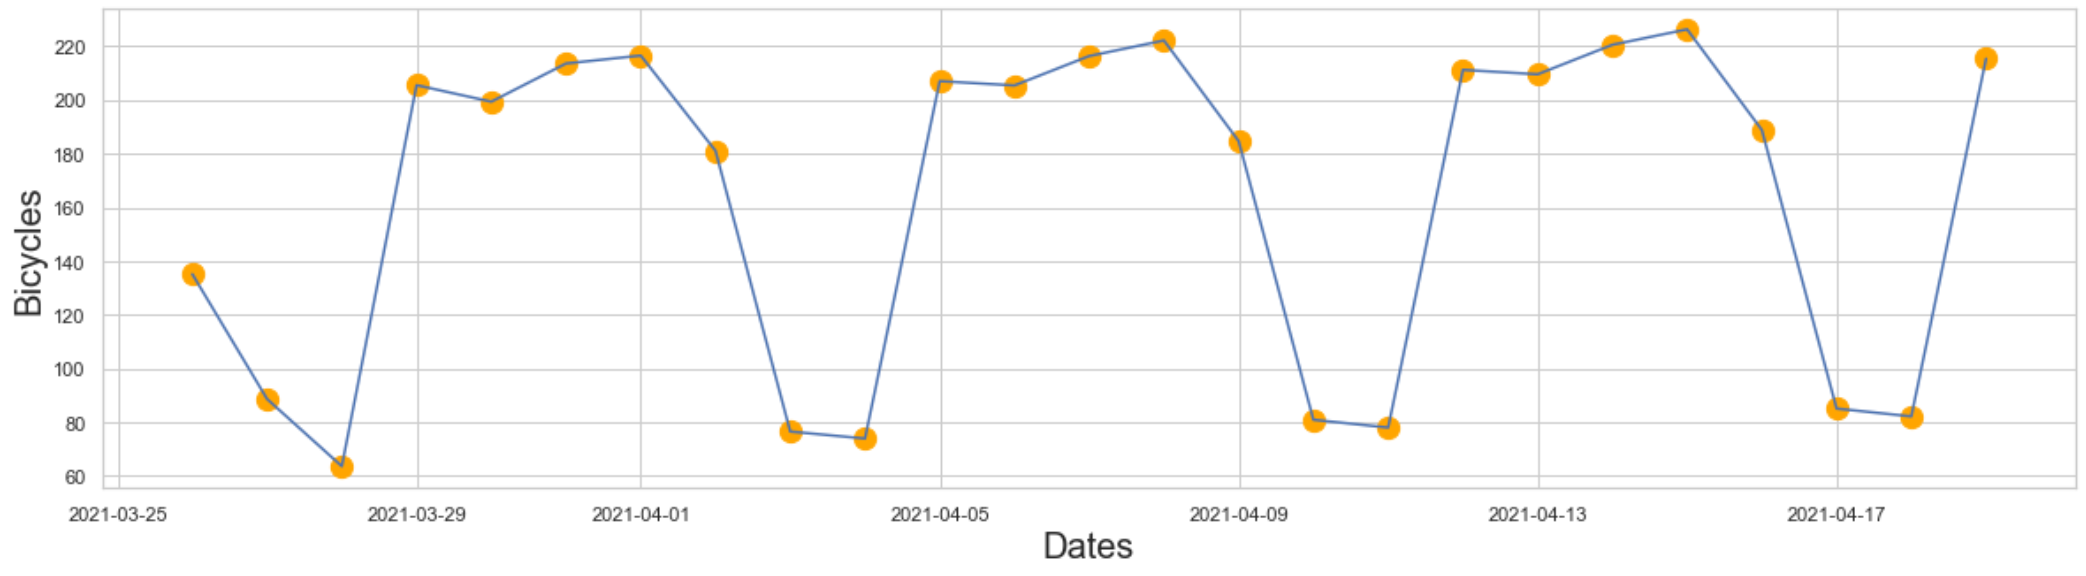
\includegraphics[scale=0.4]{data4.png}
\end{figure}

La prévision du nombre de vélos passant à Albert 1$^{er}$ le 2 avril entre 00h01 et 9h00 est 181.\\

\underline{Lien Git :}\\ \\ \par https://github.com/Stephaniujka/Bike\_Challenge\_2021/blob/master/Prediction/prediction.ipynb\\





\end{document}
